\section*{Dépendances externes}
\addcontentsline{toc}{section}{\protect\numberline{}Dépendances externes}

	Avant même de concevoir un logiciel, il faut au préalable le penser, ainsi que définir ses besoins et ses diférentes fonctionnalités. Dans cette optique, notre cahier des charges nous imposait de concevoir l'application en \texttt{langage C}. Ce langage ne fût pas choisi pour ses performances dans la conception d'applications réseau, mais plutôt dans une optique pédagogique. En effet, il est moins évident de programmer des échanges entre clients et serveur en \texttt{langage C} plutôt qu'en \texttt{Java} ou en \texttt{C++}, où tout est mis à disposition pour aider le programmeur.

\vspace{0.5cm}

	En ce qui concerne la partie graphique de l'application, nous avons choisi d'utiliser le \texttt{CSFML} qui est le binding officiel de la SFML pour le langage C. La \texttt{SFML} étant une interface de programmation destinée à construire des jeux vidéo ou des programmes interactifs en \texttt{C++}.

\section*{Fonctionnalités du logiciel}
\addcontentsline{toc}{section}{\protect\numberline{}Fonctionnalités du logiciel}

	Pour ce projet, aucune fonctionnalité ne nous a été imposée, excepté qu'il fallait créer une application de type \textit{client}/\textit{serveur}. Pour ce faire, nous avons décidé d'utiliser le serveur en tant que moteur du jeu et les clients en tant que joueurs. Le serveur est capable de gérer jusqu'à XXX parties en simultané (si la machine qui le lance est assez puissante), et chaque partie comprend de 2 à 4 joueurs. Pour des raisons de simplicité, de performance et de fluidité, une partie se déroule en tour par tour (un client doit attendre son tour pour jouer). 

\vspace{0.5cm}

	Les règles du jeux sont simple, pour gagner, un joueur doit éliminer tous les autres en réduidant leur point de vie à 0. Pour ce faire, chaque joueur dispose au départ de 3 points de vie, et peut poser jusqu'à 3 bombes en même temps sur la carte. Lorsqu'une bombe est posée, elle change d'état progressivement jusqu'à exploser.
Un joueur peut être blessé par ces propres bombes ?????
Lorsqu'une bombe explose, les joueurs présent autour de la bombe sont touchés et perdent un point de vie ?????

\section*{Interface graphique}
\addcontentsline{toc}{section}{\protect\numberline{}Interface graphique}

	En ce qui concerne l'interface graphique, nous l'avons entièrement construite à l'aide de la \texttt{CSFML}. Il s'agit d'un ensemble d'éléments graphiques, appelés \textit{sprite} que l'on place dans une fenêtre. Nous avons créé l'intégralité de nos sprite nous même à l'aide d'une base de donnée libre d'images et d'un logiciel infographique. 
\vspace{0.5cm}

\noindent{Voici quelques exemples de sprites : \\
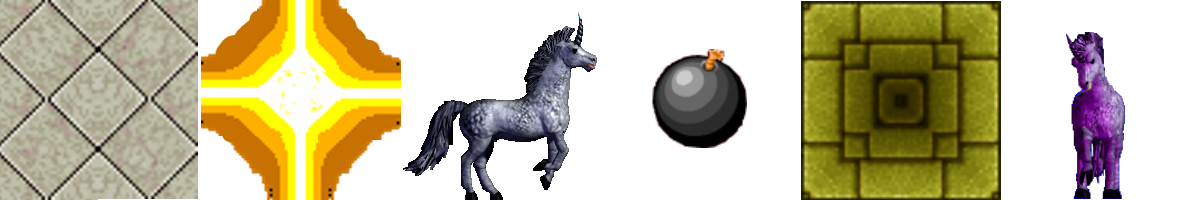
\includegraphics[width=1\textwidth]{Figures/exempleSprite.png}}
\vspace{0.5cm}

\noindent{Voici la carte créée avec les sprites : \\
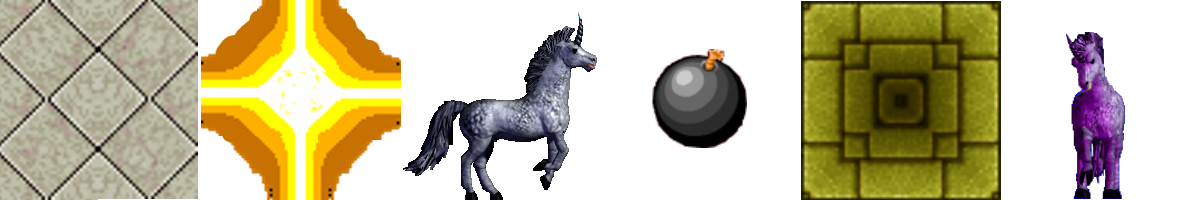
\includegraphics[width=1\textwidth]{Figures/exempleSprite.png}}

